\documentclass[journal,article,submit,pdftex]{Definitions/mdpi}

\usepackage{tabularx}
\usepackage{caption}

\firstpage{1}
\setlength{\headheight}{20.0pt}
\makeatletter
\setcounter{page}{\@firstpage}
\makeatother

\pubvolume{1}
\issuenum{1}
\articlenumber{0}
\pubyear{2025}
\copyrightyear{2025}

\datereceived{}
\daterevised{} % Comment out if no revised date
\dateaccepted{}
\datepublished{}

\hreflink{https://www.mdpi.com/journal/iot} % If needed, change journal link

\Title{Implementación de laboratorio de física para ingeniería mediante retrofitting con tecnologías IoT en un entorno de aprendizaje híbrido.}

\Author{Walter Santiago Sosa Mej\'ia}
\AuthorNames{Walter Santiago Sosa Mej\'ia}
\AuthorCitation{Sosa Mej\'ia, W.S.}

\address{%
\quad Pontificia Universidad Cat\'olica del Ecuador, Sede Esmeraldas; wssosa@pucese.edu.ec}

%-------------------------------------------------
% RESUMEN
%-------------------------------------------------

\abstract{La modernización de laboratorios de física en contextos de recursos limitados presenta desafíos significativos. Este artículo presenta el diseño y validación de un sistema de laboratorio remoto para el estudio del Movimiento Rectilíneo Uniformemente Acelerado (MRUA), implementado mediante una estrategia de \textit{retrofitting} con tecnologías de Internet de las Cosas (IoT) sobre equipamiento preexistente. La arquitectura propuesta utiliza un microcontrolador ESP32, en adelante denominado módulo de control, y sensores infrarrojos para la captura de datos, gestionados a través de una interfaz web que permite el control y visualización en tiempo real. Para validar el sistema, se realizó un estudio comparativo con 70 ensayos (35 en modalidad remota y 35 en presencial). Los resultados demuestran que el prototipo remoto alcanza una precisión cinemática comparable al montaje tradicional, manteniendo una alta estabilidad en las mediciones de tiempo, velocidad y aceleración, con desviaciones estándar controladas. Se concluye que la metodología de \textit{retrofitting} IoT es una solución viable y escalable para democratizar el acceso a la educación experimental de alta calidad en entornos híbridos, sin requerir grandes inversiones en infraestructura.}

\keyword{Retrofitting; Internet of Things; Remote laboratories; MRUA; Low-cost instrumentation; Cloud services; Engineering education}

\begin{document}

%-------------------------------------------------
% INTRODUCCION
%-------------------------------------------------

\section{Introduction}

Los laboratorios de f\'isica constituyen un componente esencial para la verificaci\'on experimental de leyes y modelos, as\'i como para la validaci\'on de sistemas de medici\'on y control. Tradicionalmente, estos entornos han operado de forma estrictamente presencial, con instrumentaci\'on anal\'ogica o digital que requiere la presencia f\'isica del usuario en el laboratorio. Sin embargo, la creciente digitalizaci\'on de la infraestructura cient\'ifica y el desarrollo de arquitecturas ciberf\'isicas han impulsado el dise\~no de plataformas que permiten operar, monitorear y automatizar experimentos de manera remota y distribuida \cite{r1}. La pandemia de COVID-19 reforz\'o esta tendencia al mostrar las limitaciones de los montajes dependientes exclusivamente de la presencia local, acelerando la adopci\'on de laboratorios remotos y sistemas de instrumentaci\'on conectados a la nube \cite{r2}.

En este contexto, se hace evidente un problema recurrente: muchos laboratorios de f\'isica contin\'uan dependiendo de montajes centrados en la operaci\'on presencial, con escaso nivel de automatizaci\'on, sin mecanismos de acceso remoto y con dificultades para registrar y gestionar datos de manera sistem\'atica. Esta situaci\'on es particularmente notoria en Am\'erica Latina, donde numerosos laboratorios operan con instrumentaci\'on en servicio desde hace varios a\~nos y con recursos limitados para renovar equipos o incorporar soluciones de conectividad avanzadas \cite{r3,r4}. El laboratorio de f\'isica de la Pontificia Universidad Cat\'olica del Ecuador sede Esmeraldas, constituye un ejemplo representativo: dispone de pistas tipo juguete, carritos de baja fricci\'on y elementos de medici\'on convencionales para experimentos de cinem\'atica y din\'amica, pero carece de capacidades de automatizaci\'on y de acceso remoto. En este escenario, dise\~nar arquitecturas que permitan \textit{retrofitting} de montajes existentes con tecnolog\'ias IoT de bajo coste se vuelve una necesidad t\'ecnica y operativa.

\subsection{Related Work and Research Gap}

La literatura reciente evidencia avances significativos en la modernización de laboratorios de física mediante tecnologías digitales, particularmente a través de laboratorios remotos, híbridos y estrategias de \textit{retrofitting} basadas en IoT. Estudios como los de Lahme \textit{et al.} \cite{r1} documentan el incremento en el uso de microcontroladores, sensores y plataformas digitales en cursos de laboratorio, destacando tanto su potencial como las barreras técnicas asociadas a su adopción. De manera complementaria, trabajos orientados al control remoto de sistemas físicos, como los presentados por Guerrero-Osuna \textit{et al.} \cite{r4} y Fuertes \textit{et al.} \cite{r3}, demuestran la viabilidad de integrar hardware embebido, servicios en la nube e interfaces web para operar experimentos reales con tiempos de respuesta adecuados.

En el contexto específico del \textit{retrofitting} de equipamiento existente, Viswanadh \textit{et al.} \cite{r2} proponen arquitecturas de bajo coste que permiten instrumentar montajes de laboratorio preexistentes sin modificaciones estructurales, mientras que Lustig \textit{et al.} \cite{r5} introducen plataformas modulares que desacoplan el hardware experimental de los servicios de acceso y visualización. Por su parte, Zhao \cite{r6} revisa extensivamente soluciones basadas en sensores de uso masivo y análisis de video, mostrando que es posible obtener mediciones de calidad razonable empleando dispositivos accesibles y ampliamente disponibles.

No obstante, a pesar de estos aportes, se identifican varias limitaciones en la literatura existente. En primer lugar, muchos trabajos se centran en la demostración funcional de plataformas remotas o en evaluaciones de usabilidad, sin profundizar en la validación cuantitativa de la fidelidad experimental frente a montajes presenciales de referencia. En segundo lugar, existe una carencia de estudios que analicen de manera sistemática el desempeño técnico de experimentos clásicos de física como los de cinemática cuando son ejecutados en modalidad remota, considerando métricas como error en tiempos de detección, coherencia interna de los datos y estabilidad del sistema. Finalmente, son escasos los estudios que abordan estas problemáticas en contextos de recursos limitados, donde la reutilización de equipamiento existente mediante \textit{retrofitting} resulta especialmente relevante.

En este marco, el presente trabajo se diferencia al proponer y validar un modelo de laboratorio híbrido de física basado en \textit{retrofitting} IoT. Para contextualizar nuestra contribución dentro de las arquitecturas modernas de IoT, se adopta el enfoque de capas propuesto por Dizdarevic y Jukan \cite{r7}, quienes destacan la importancia de integrar capacidades de computación en el borde (\textit{Edge}) y en la nube (\textit{Cloud}) para reducir la latencia en entornos educativos, una lección que hemos aplicado mediante el uso del dispositivo de control para el procesamiento en el borde. Asimismo, para asegurar la continuidad operativa y la accesibilidad universal, seguimos los principios de Azad \cite{r8} sobre el despliegue de laboratorios remotos basados en IoT, garantizando que el sistema sea robusto frente a desconexiones. Finalmente, la validación de nuestro sistema se alinea con la metodología de "gemelos digitales" descrita por Palmer \textit{et al.} \cite{r9}, utilizando la comparación directa entre los datos físicos del sensor (el "gemelo real") y el modelo teórico esperado, asegurando así una verificación cuantitativa rigurosa.

%-------------------------------------------------
% MATERIALES Y METODOS
%-------------------------------------------------

\section{Materials and Methods}
\label{sec:metodos}

\subsection{Dise\~no de la investigaci\'on}

La investigaci\'on se plante\'o como un estudio aplicado de tipo t\'ecnico, orientado al dise\~no, construcci\'on y validaci\'on de un prototipo de laboratorio de f\'isica controlado a distancia mediante tecnolog\'ias IoT. Se adopt\'o un enfoque cuantitativo de alcance descriptivo, ya que las variables centrales de an\'alisis corresponden a magnitudes f\'isicas medibles (tiempos de detecci\'on, eventos registrados, ocurrencia de fallos) obtenidas a partir de registros instrumentales del sistema, que posteriormente se describen y comparan sin intervenir sobre grupos de participantes humanos. El enfoque metodol\'ogico se aline\'o con la l\'ogica de la \textit{Design Science Research} (DSR), en la que el objetivo central es construir un artefacto tecnol\'ogico y evaluarlo de forma sistem\'atica \cite{r11}, y tom\'o como referencia general los procesos de ciclo de vida de sistemas descritos en la norma ISO/IEC~15288 para organizar las fases de requisitos, dise\~no, implementaci\'on, integraci\'on y operaci\'on del prototipo \cite{r12}.

A partir de este marco se defini\'o que el alcance de la presente investigaci\'on se concentrar\'ia en la evaluaci\'on t\'ecnica del experimento de movimiento rectil\'ineo uniformemente acelerado (MRUA), espec\'ificamente en la exactitud y consistencia de las variables f\'isicas medidas y calculadas por el sistema remoto para dicho experimento frente a un montaje presencial de referencia equivalente.

%-------------------------------------------------
\subsection{Hardware y software utilizados}

Para garantizar una presentaci\'on clara y replicable, los materiales utilizados se agrupan en dos tablas: componentes de hardware (Tabla~\ref{tab:hardware}) y herramientas de software (Tabla~\ref{tab:software}). La Figura~\ref{fig:arquitectura} resume c\'omo se integran estos elementos en la arquitectura general del sistema.

\begin{table}[H]
	\caption{Componentes de hardware del prototipo de laboratorio h\'ibrido de f\'isica basado en tecnolog\'ias IoT.\label{tab:hardware}}
	\small
	\begin{adjustwidth}{-\extralength}{0cm}
		\renewcommand{\arraystretch}{1.5}
		\renewcommand{\tabularxcolumn}[1]{m{#1}}
		\begin{tabularx}{\fulllength}{>{\raggedright\arraybackslash}m{4.5cm}Xc}
			\toprule
			\textbf{Categor\'ia del dispositivo} & \textbf{Especificaci\'on t\'ecnica consolidada} & \textbf{Referencias} \\
			\midrule
			Sistema experimental mec\'anico & Pista tipo Hot Wheels\textsuperscript{\textregistered} utilizada como riel de movimiento rectil\'ineo y carrito de baja fricci\'on adaptado para pr\'acticas de cinem\'atica & \cite{r13, r14} \\
			Sistema de sensado y adquisici\'on de datos & Cuatro sensores infrarrojos para detecci\'on de paso y medici\'on de tiempo & \cite{r15} \\
			Unidad de control y procesamiento IoT & Módulo de control DevKit (30 pines, USB-C, conectividad WiFi y Bluetooth integrada) & \cite{r16} \\
			Estructura mec\'anica y soporte f\'isico & Soportes, refuerzos y conjuntos mec\'anicos impresos en 3D para montaje de sensores, actuadores y elementos estructurales & \cite{r17, r18, r19, r20} \\
			Actuadores y control de movimiento & Servomotor SG90 (180\textdegree), motor paso a paso bipolar NEMA 17 y m\'odulo puente H L298N para control de movimiento & \cite{r21, r22, r23} \\
			Interfaz de usuario local & Pantalla LCD 20x4 con interfaz I\textsuperscript{2}C y pulsador mec\'anico para interacci\'on local & \cite{r24, r25} \\
			Comunicaci\'on y conectividad & Est\'andar inal\'ambrico IEEE 802.11 (WiFi), cable USB tipo C y cables Dupont para interconexi\'on el\'ectrica & \cite{r26, r27, r28} \\
			Sistema de alimentaci\'on y protecci\'on & Adaptador AC--DC 12 V / 1 A y caja pl\'astica de protecci\'on para proyectos electr\'onicos (135 $\times$ 75 $\times$ 40 mm) & \cite{r29, r30} \\
			Sistema de visualizaci\'on remota & Webcam Insta360 Link con resoluci\'on 4K y funciones de seguimiento asistidas por IA & \cite{r31} \\
			Servidor y gesti\'on del sistema IoT & Raspberry Pi 4 Model B para gesti\'on de comunicaciones, almacenamiento y monitoreo del sistema & \cite{r32} \\
			\bottomrule
		\end{tabularx}
	\end{adjustwidth}
\end{table}


\begin{table}[H]
	\caption{Herramientas de software utilizadas en el sistema del laboratorio h\'ibrido de f\'isica basado en IoT.\label{tab:software}}
	\small
	\begin{adjustwidth}{-\extralength}{0cm}
		\renewcommand{\arraystretch}{1.5}
		\renewcommand{\tabularxcolumn}[1]{m{#1}}
		\begin{tabularx}{\fulllength}{>{\raggedright\arraybackslash}m{3.5cm}X>{\centering\arraybackslash}m{3.5cm}c}
			\toprule
			\textbf{Capa del sistema} & \textbf{Herramientas de software} & \textbf{Versiones} & \textbf{Referencias} \\
			\midrule
			Comunicaci\'on IoT & EMQX, MQTTX Desktop & 5.10.2; 1.12.1 & \cite{r33, r34} \\
			Backend y servicios & Node.js (LTS), Express & 24.11.1; 5.1.0 & \cite{r35, r36} \\
			Persistencia de datos & MongoDB Server, MongoDB Driver, Mongoose & 8.2.2; 6.3.0; 8.5.1 & \cite{r37, r38} \\
			Frontend y visualizaci\'on & Next.js, React & 16.0; 19.2.0 & \cite{r39, r40} \\
			Desarrollo embebido & Arduino IDE & 2.3.4 & \cite{r41} \\
			Lenguajes y soporte & Python & 3.14.1 & \cite{r42} \\
			\bottomrule
		\end{tabularx}
	\end{adjustwidth}
\end{table}

\subsection{Arquitectura general del sistema}

La arquitectura general del sistema se organiza en tres capas bien diferenciadas \cite{r10} (Figura~\ref{fig:arquitectura}). La Capa~1 agrupa los elementos de percepci\'on del experimento, incluyendo el carrito de laboratorio para MRUA, la pista, los cuatro sensores infrarrojos, la c\'amara del experimento y el módulo de control, que se encarga de adquirir las se\~nales de los sensores y enviarlas mediante MQTT sobre WiFi. La Capa~2 corresponde a la red local y al servidor, formada por el router WiFi o punto de acceso y la Raspberry~Pi, donde se ejecutan el broker EMQX, el servidor de video y la API web que procesa los datos. Finalmente, la Capa~3 incluye la interfaz de usuario basada en p\'agina web, desde la cual el profesor y el estudiante pueden visualizar tablas de datos y gr\'aficas de posici\'on, velocidad y aceleraci\'on, as\'i como observar el video del experimento y enviar comandos de control al sistema.


\begin{figure}[H]
\centering
\includegraphics[width=\textwidth]{figures/fig1_arquitectura_labfisica.png}
\caption{Arquitectura basada en tres capas del laboratorio de f\'isica con \textit{retrofitting} IoT. Diagrama elaborado siguiendo el modelo fundamental de tres capas \cite{r10} con la herramienta Eraser~\cite{r43}.}
\label{fig:arquitectura}
\end{figure}

\begin{figure}[H]
\centering
\includegraphics[width=0.8\textwidth]{figures/Hardware connection diagram of the proposed prototype.png}
\caption{Esquema del m\'odulo de control. Imagen generada con la asistencia de ChatGPT \cite{r44}.}
\label{fig:hardware_connection}
\end{figure}

\begin{table}[H]
	\caption{Conexiones detalladas del sistema y asignaci\'on de pines del módulo de control.\label{tab:connections}}
	\small
	\begin{adjustwidth}{-\extralength}{0cm}
		\renewcommand{\arraystretch}{1.3}
		\renewcommand{\tabularxcolumn}[1]{m{#1}}
		\begin{tabularx}{\fulllength}{clXccc}
			\toprule
			\textbf{Nº} & \textbf{Componente} & \textbf{Funci\'on en el experimento} & \textbf{Pin m\'od. control} & \textbf{Tipo de se\~nal} & \textbf{Alimentaci\'on} \\
			\midrule
			1  & Sensor S1      & Detecci\'on inicio del movimiento         & GPIO 15 & Entrada digital (PULLUP) & 5 V / GND    \\
			2  & Sensor S2      & Detecci\'on tramo intermedio 1            & GPIO 25 & Entrada digital (PULLUP) & 5 V / GND    \\
			3  & Sensor S3      & Detecci\'on tramo intermedio 2            & GPIO 12 & Entrada digital (PULLUP) & 5 V / GND    \\
			4  & Sensor S4      & Detecci\'on final del recorrido           & GPIO 13 & Entrada digital (PULLUP) & 5 V / GND    \\
			5  & Bot\'on manual   & Inicio / cancelaci\'on del experimento    & GPIO 18 & Entrada digital (PULLUP) & GND          \\
			6  & Servo motor    & Empuje / liberaci\'on inicial del carrito & GPIO 5  & PWM                            & 5 V / GND    \\
			7  & L298N – ENA    & Control de aceleraci\'on del motor (NRUA) & GPIO 14 & PWM                            & 5 V / GND    \\
			8  & L298N – IN1    & Direcci\'on del motor DC                  & GPIO 27 & Salida digital                 & —            \\
			9  & L298N – IN2    & Direcci\'on del motor DC                  & GPIO 26 & Salida digital                 & —            \\
			10 & LCD 16$\times$2 – SDA & Comunicaci\'on I2C (datos)                & GPIO 21 & I2C                            & 5 V / GND    \\
			11 & LCD 16$\times$2 – SCL & Comunicaci\'on I2C (reloj)                & GPIO 22 & I2C                            & 5 V / GND    \\
			12 & Motor DC       & Generaci\'on del movimiento acelerado     & L298N   & Potencia                       & 11–12 V  \\
			13 & Tierra com\'un   & Referencia el\'ectrica del sistema        & GND     & —                              & Com\'un        \\
			\bottomrule
		\end{tabularx}
	\end{adjustwidth}
\end{table}



\subsection{Poblaci\'on, muestra y entorno experimental}

En este estudio no se trabaja con una poblaci\'on de sujetos humanos ni con unidades organizacionales, sino con un sistema f\'isico instrumentado cuyo comportamiento se eval\'ua desde una perspectiva t\'ecnica. Por este motivo, en lugar de definir una poblaci\'on y muestra en el sentido cl\'asico de la investigaci\'on cuantitativa, esta subsecci\'on se centra en describir el entorno experimental del laboratorio y la forma en que se planificaron los ensayos realizados sobre el montaje. En total, se ejecutaron 70 ensayos, correspondientes a 35 pruebas en modalidad presencial y 35 en modalidad remota.

El experimento se llev\'o a cabo en el laboratorio de f\'isica de la Pontificia Universidad Cat\'olica del Ecuador sede Esmeraldas, que dispone de una mesa de trabajo nivelada, acceso a red el\'ectrica regulada y conectividad de red local mediante un punto de acceso WiFi. En este espacio se instal\'o la pista tipo Hot Wheels\textsuperscript{\textregistered} \cite{r13}, el carrito de laboratorio de baja fricci\'on \cite{r14}, los cuatro sensores infrarrojos \cite{r15}, el módulo de control \cite{r16} y la c\'amara Insta360 Link \cite{r31}, conformando el montaje f\'isico del experimento de MRUA. La Raspberry~Pi~4 utilizada como servidor IoT \cite{r32} se ubic\'o en el mismo laboratorio y se conect\'o tanto al punto de acceso WiFi \cite{r27} como a la red cableada institucional.

%-------------------------------------------------
\subsection{Procedimiento de implementaci\'on}

El procedimiento seguido para desarrollar y evaluar el prototipo se organiz\'o en cuatro momentos, coherentes con los objetivos espec\'ificos del estudio: dise\~no del sistema y definici\'on de la arquitectura IoT del laboratorio remoto, implementaci\'on del hardware y del software, configuraci\'on del entorno experimental con ejecuci\'on de ensayos en modo remoto y presencial, y validaci\'on t\'ecnica del funcionamiento del prototipo.

En primer lugar, se realiz\'o un levantamiento de requisitos junto con el docente responsable de la asignatura de F\'isica, considerado experto en el experimento de MRUA. En esta etapa se identificaron los eventos que deb\'ia registrar el sistema (paso del carrito por cada sensor), la informaci\'on m\'inima necesaria para describir el experimento y las condiciones de montaje aceptables en el laboratorio. A partir de estos insumos se defini\'o la arquitectura IoT del laboratorio remoto, especificando los componentes de hardware, los servicios de software y el flujo de datos entre el ESP32, el servidor MQTT, el backend y la aplicaci\'on web. Las decisiones de dise\~no se documentaron en los archivos \texttt{README} del repositorio p\'ublico \textit{RemotePhysicsLab} \cite{r45}, en las carpetas de \texttt{frontend} y \texttt{backend}.

En una segunda fase se llev\'o a cabo la implementaci\'on del prototipo IoT (Figura~\ref{fig:arquitectura}). Se construy\'o el montaje f\'isico de la pista y se instalaron los sensores infrarrojos en posiciones fijas a lo largo del recorrido del carrito. El módulo de control se program\'o utilizando el entorno Arduino IDE para leer el estado de los sensores y enviar mensajes MQTT con marcas de tiempo hacia el servidor MQTT desplegado en la Raspberry~Pi. De manera paralela se configur\'o la c\'amara del experimento y el servidor de video, de modo que la se\~nal pudiera ser consumida desde el navegador web. Durante esta fase se realizaron pruebas unitarias para comprobar la lectura correcta de los sensores, la conectividad WiFi, la publicaci\'on en los t\'opicos MQTT definidos y la recepci\'on continua de la se\~nal de video.

A continuaci\'on se configur\'o el entorno experimental y se procedi\'o a la ejecuci\'on de los ensayos. Se fijaron el punto de partida del carrito, la inclinaci\'on de la pista y las posiciones de los sensores, manteniendo estos par\'ametros constantes en todas las pruebas. Con esta configuraci\'on se realizaron series de ensayos en dos modalidades: por una parte, la operaci\'on remota mediante la interfaz web del laboratorio, en la que el usuario activaba el experimento, observaba el movimiento del carrito a trav\'es del video en tiempo casi real y los tiempos de detecci\'on quedaban registrados autom\'aticamente en el sistema; y, por otra, la operaci\'on presencial utilizando un montaje de referencia sin el componente IoT, que sirvi\'o como l\'inea base para comparar las mediciones de tiempo y las magnitudes cinem\'aticas derivadas. En ambas modalidades se repiti\'o el experimento varias veces para obtener un conjunto suficiente de registros.

Finalmente, se realiz\'o la validaci\'on t\'ecnica del prototipo. Para ello se recopilaron los datos generados por el sistema remoto y por el montaje presencial, organiz\'andolos en tablas comparativas por sensor y por repetici\'on. A partir de estas tablas se evalu\'o la coincidencia de los tiempos de detecci\'on entre ambas modalidades, se verific\'o si el sistema remoto registraba todos los eventos esperados en cada recorrido del carrito y se documentaron de forma cualitativa las incidencias relacionadas con la estabilidad del sistema, tales como ca\'idas de servicio, desconexiones o necesidad de reinicio durante las sesiones de prueba. Este procedimiento permiti\'o comprobar en qu\'e medida el prototipo reproduce de manera consistente el experimento de MRUA en modalidad remota en comparaci\'on con el montaje de referencia presencial.

\begin{figure}[H]
\centering
\includegraphics[width=\textwidth]{figures/Experimental procedure flowchart.png}
\caption{Flujo de datos durante la operaci\'on del laboratorio. 
Las lecturas de los sensores infrarrojos asociadas al paso del carrito son enviadas por el módulo de control al servidor MQTT mediante MQTT. 
El backend procesa los mensajes, los registra en MongoDB y los expone a la aplicaci\'on web, que a su vez presenta los datos y el video del experimento al usuario. Fue elaborada con la herramienta de diagramaci\'on asistida por IA Eraser\cite{r43}}
\label{fig:flujo-datos}
\end{figure}

%-------------------------------------------------
\subsection{Métricas de evaluación}

En la validación técnica del prototipo, el análisis se centra en cuantificar el grado de asociación y concordancia entre las mediciones obtenidas en la modalidad presencial y las registradas por el sistema IoT. El objetivo es determinar si la instrumentación tecnológica basada en \textit{retrofitting} es capaz de replicar la estabilidad y precisión del montaje tradicional. Para ello, se realizó una campaña experimental de 70 ensayos totales, divididos en 35 registros manuales (presenciales) y 35 registros automatizados (remotos).

Como métrica fundamental de desempeño, se adopta el coeficiente de correlación de Pearson (\(r\)), el cual permite evaluar la fidelidad con la que el laboratorio remoto reproduce el comportamiento observado en el montaje físico de referencia. Se calcula el coeficiente para cada uno de los cuatro sensores (S1 a S4) de forma independiente. Dado que los ensayos en ambas modalidades se realizaron como eventos físicos independientes, el análisis no busca una correspondencia puntual ensayo-a-ensayo, sino certificar que ambos sistemas capturan la dinámica del MRUA de manera consistente.

El coeficiente de correlación se define mediante la siguiente ecuación:

\begin{equation}
r = \frac{\sum_{i=1}^{n} (x_i - \bar{x})(y_i - \bar{y})}{\sqrt{\sum_{i=1}^{n} (x_i - \bar{x})^2} \sqrt{\sum_{i=1}^{n} (y_i - \bar{y})^2}}
\label{eq:pearson}
\end{equation}

Donde \(x_i\) representa los tiempos medidos en la modalidad presencial (referencia manual) y \(y_i\) los tiempos medidos en la modalidad remota (IoT) para una serie de \(n=35\) ensayos por modalidad, con sus respectivos promedios \(\bar{x}\) y \(\bar{y}\). Un valor de \(r\) próximo a 1 valida que la instrumentación IoT captura la variabilidad natural del fenómeno cinemático con una fidelidad equivalente al cronometraje presencial.



%-------------------------------------------------

\subsection{M\'etodos de an\'alisis de datos}

Los datos registrados por el prototipo IoT (modalidad h\'ibrida) y por el montaje presencial de referencia se exportaron en forma de archivos de texto estructurados, que contienen las marcas de tiempo asociadas al paso del carrito por cada sensor y la configuraci\'on de cada ensayo. Estos registros se organizaron en hojas de c\'alculo y posteriormente se procesaron mediante scripts desarrollados en Python~3.14.1\cite{r42}.

El an\'alisis se centr\'o en la consistencia de los tiempos de paso por sensor y en el c\'alculo de la correlaci\'on de Pearson entre las modalidades h\'ibrida y presencial. Se generaron gr\'aficos de dispersi\'on para visualizar la proximidad entre las mediciones obtenidas y detectar posibles desviaciones del prototipo. Los resultados num\'ericos y gr\'aficos se presentan y discuten en la secci\'on de Resultados.
En una primera etapa, los datos de ambas modalidades se integraron en tablas comparativas que agrupan, por ensayo, los tiempos de paso registrados por el sistema h\'ibrido y por el montaje presencial. En una segunda etapa, se generaron gr\'aficos de dispersi\'on e histogramas para visualizar la proximidad entre las mediciones obtenidas en ambas modalidades y validar la consistencia del prototipo mediante el análisis de correlación.

Los resultados num\'ericos de estas comparaciones, as\'i como las tablas y gr\'aficos derivados del procesamiento en Python~3.14.1, se presentan y discuten en la secci\'on de Resultados, donde se analiza en detalle la concordancia del laboratorio h\'ibrido frente al montaje presencial de referencia.


%-------------------------------------------------
\subsection{Control de validez y confiabilidad}

El control de validez y confiabilidad se enfoc\'o en asegurar que las mediciones realizadas por el prototipo IoT fueran coherentes con el comportamiento f\'isico esperado del experimento de MRUA y comparables con las obtenidas en el montaje presencial de referencia.

En primer lugar, se verific\'o la validez de medici\'on mediante pruebas espec\'ificas de detecci\'on del carrito por parte de los sensores infrarrojos. Para ello, se realizaron ensayos de prueba en los que el carrito se desplazaba de forma controlada a lo largo de la pista, observando en tiempo real el estado de las entradas digitales del módulo de control y los mensajes publicados v\'ia MQTT. Se ajustaron la altura y la orientaci\'on de cada sensor hasta garantizar que el paso del carrito generara transiciones limpias de se\~nal (activo/inactivo) sin disparos espurios por ruido ambiental o reflexiones indeseadas. La pista utilizada tiene una longitud efectiva de 160~cm, sobre la cual se distribuyeron los cuatro sensores de detecci\'on a intervalos de 53.2~cm, lo que permiti\'o contar con distancias bien definidas para el c\'alculo de velocidades y aceleraciones a partir de los tiempos de paso.

Adicionalmente, se cuid\'o la medici\'on de las distancias fijas entre sensores empleando una cinta m\'etrica convencional con resoluci\'on adecuada para el experimento, de modo que los c\'alculos cinem\'aticos derivados (velocidad y aceleraci\'on promedio) se basaran en valores de referencia consistentes. El montaje presencial del laboratorio se utiliz\'o como l\'inea base para contrastar los tiempos y magnitudes cinem\'aticas obtenidos con el prototipo IoT, constituyendo as\'i un punto de referencia para la validez externa de las mediciones.

En cuanto a la confiabilidad y repetibilidad, se realizaron un total de 70 ensayos repetidos (35 presenciales y 35 remotos) bajo la misma configuraci\'on del montaje (misma inclinaci\'on de la pista, misma posici\'on inicial del carrito y misma ubicaci\'on de los sensores) tanto en la modalidad presencial como en la modalidad h\'ibrida. A partir de estos ensayos se analiz\'o la variabilidad de los tiempos de paso y de las aceleraciones estimadas, empleando estad\'isticas descriptivas b\'asicas (media y desviaci\'on est\'andar) como indicador de la estabilidad de las mediciones. Los registros que presentaron anomal\'ias evidentes (por ejemplo, fallos de detecci\'on, interrupciones de comunicaci\'on o errores manifiestos de lanzamiento) se descartaron expl\'icitamente del an\'alisis comparativo y se documentaron como eventos at\'ipicos, con el fin de no sesgar las conclusiones sobre el desempe\~no normal del sistema.

Para reducir amenazas a la validez interna, el experimento se desarroll\'o en condiciones controladas: la pista y los sensores se mantuvieron fijos sobre una misma mesa de trabajo, se evit\'o manipular el montaje entre series de ensayos y se procur\'o mantener una iluminaci\'on estable en el laboratorio, de manera que no se introdujeran variaciones relevantes en la respuesta de los sensores ni en la calidad de la se\~nal de video. En el plano de la instrumentaci\'on, el módulo de control registr\'o localmente las marcas de tiempo asociadas a cada evento de detecci\'on, de modo que la latencia de red afectara solo a la visualizaci\'on remota y no al sellado temporal de los datos f\'isicos. La comunicaci\'on con el servidor MQTT se supervis\'o mediante suscripciones de prueba a los t\'opicos MQTT, verificando que no se produjeran p\'erdidas sistem\'aticas de mensajes durante las sesiones de medici\'on.

Finalmente, en t\'erminos de validez externa, se reconoce que el estudio se centra en la evaluaci\'on t\'ecnica del prototipo de laboratorio h\'ibrido para un experimento concreto de din\'amica (MRUA) y en un entorno espec\'ifico (laboratorio de f\'isica de la PUCE sede Esmeraldas). No se pretende generalizar los resultados a indicadores de aprendizaje ni a percepciones de usabilidad por parte de los estudiantes, sino demostrar que la arquitectura basada en \textit{retrofitting} e IoT puede reproducir con suficiente precisi\'on y estabilidad las mediciones de un montaje presencial de referencia bajo condiciones controladas.

%-------------------------------------------------

\subsection{Reproducibilidad y \'etica}

Con el fin de facilitar la reproducibilidad del estudio, el c\'odigo fuente del prototipo de laboratorio h\'ibrido, as\'i como los archivos de configuraci\'on necesarios para desplegar el backend, el servidor MQTT y la aplicaci\'on web, se publicaron en un repositorio p\'ublico en GitHub\cite{r45}. En el archivo \texttt{README.md} se documentan los pasos para clonar el repositorio, instalar las dependencias, configurar las variables de entorno y ejecutar los servicios involucrados, junto con indicaciones sobre la versi\'on de hardware y software recomendada. De este modo, otros equipos pueden replicar la arquitectura propuesta utilizando una combinaci\'on similar de módulo de control, Raspberry~Pi, EMQX y aplicaci\'on web, o adaptar el dise\~no a sus propios laboratorios de f\'isica.

En cuanto a las consideraciones éticas e institucionales, el desarrollo y la evaluaci\'on del prototipo se realizaron con la autorizaci\'on expl\'icita de la Pontificia Universidad Cat\'olica del Ecuador sede Esmeraldas, tanto para el uso del laboratorio de f\'isica como para la menci\'on de la instituci\'on en el manuscrito. El estudio no implic\'o la recolecci\'on de datos personales ni la participaci\'on de estudiantes como sujetos de investigaci\'on, por lo que no se requiri\'o la aplicaci\'on de protocolos adicionales de consentimientos individuales. Las actividades se limitaron al uso responsable de la infraestructura del laboratorio y al registro de variables f\'isicas asociadas al experimento de MRUA.

%-------------------------------------------------
% RESULTADOS
%-------------------------------------------------

\section{Resultados}

Esta sección presenta los resultados obtenidos de la validación experimental del sistema de \textit{retrofitting} basado en IoT propuesto. El análisis se centra en la estabilidad de la captura de datos y en la correlación estadística entre las modalidades remota (IoT) y presencial (tradicional). El conjunto de datos comprende \(N=70\) ensayos independientes (35 remotos y 35 presenciales).

\subsection{Configuración experimental e implementación del prototipo}

La implementación física del prototipo integra la estructura mecánica, la capa de sensado electrónico y la unidad de control IoT. Debido a la longitud de la pista (160 cm), el montaje se muestra en secciones detalladas para observar la disposición de los componentes. En la Figura~\ref{fig:montaje_detalles} se presentan las cuatro secciones principales del recorrido: (a) inicio del recorrido, (b) tramo 2, (c) tramo 3 y (d) punto de llegada. Finalmente, una vista general del prototipo completo se observa en la Figura~\ref{fig:vista_general}. El sistema de detección consta de cuatro sensores infrarrojos distribuidos a intervalos precisos de 53.2 cm, integrados a lo largo de la estructura para capturar el tiempo total desde la liberación automatizada del carrito hasta el final del recorrido.
\begin{figure}[H]
\centering
\subfloat[]{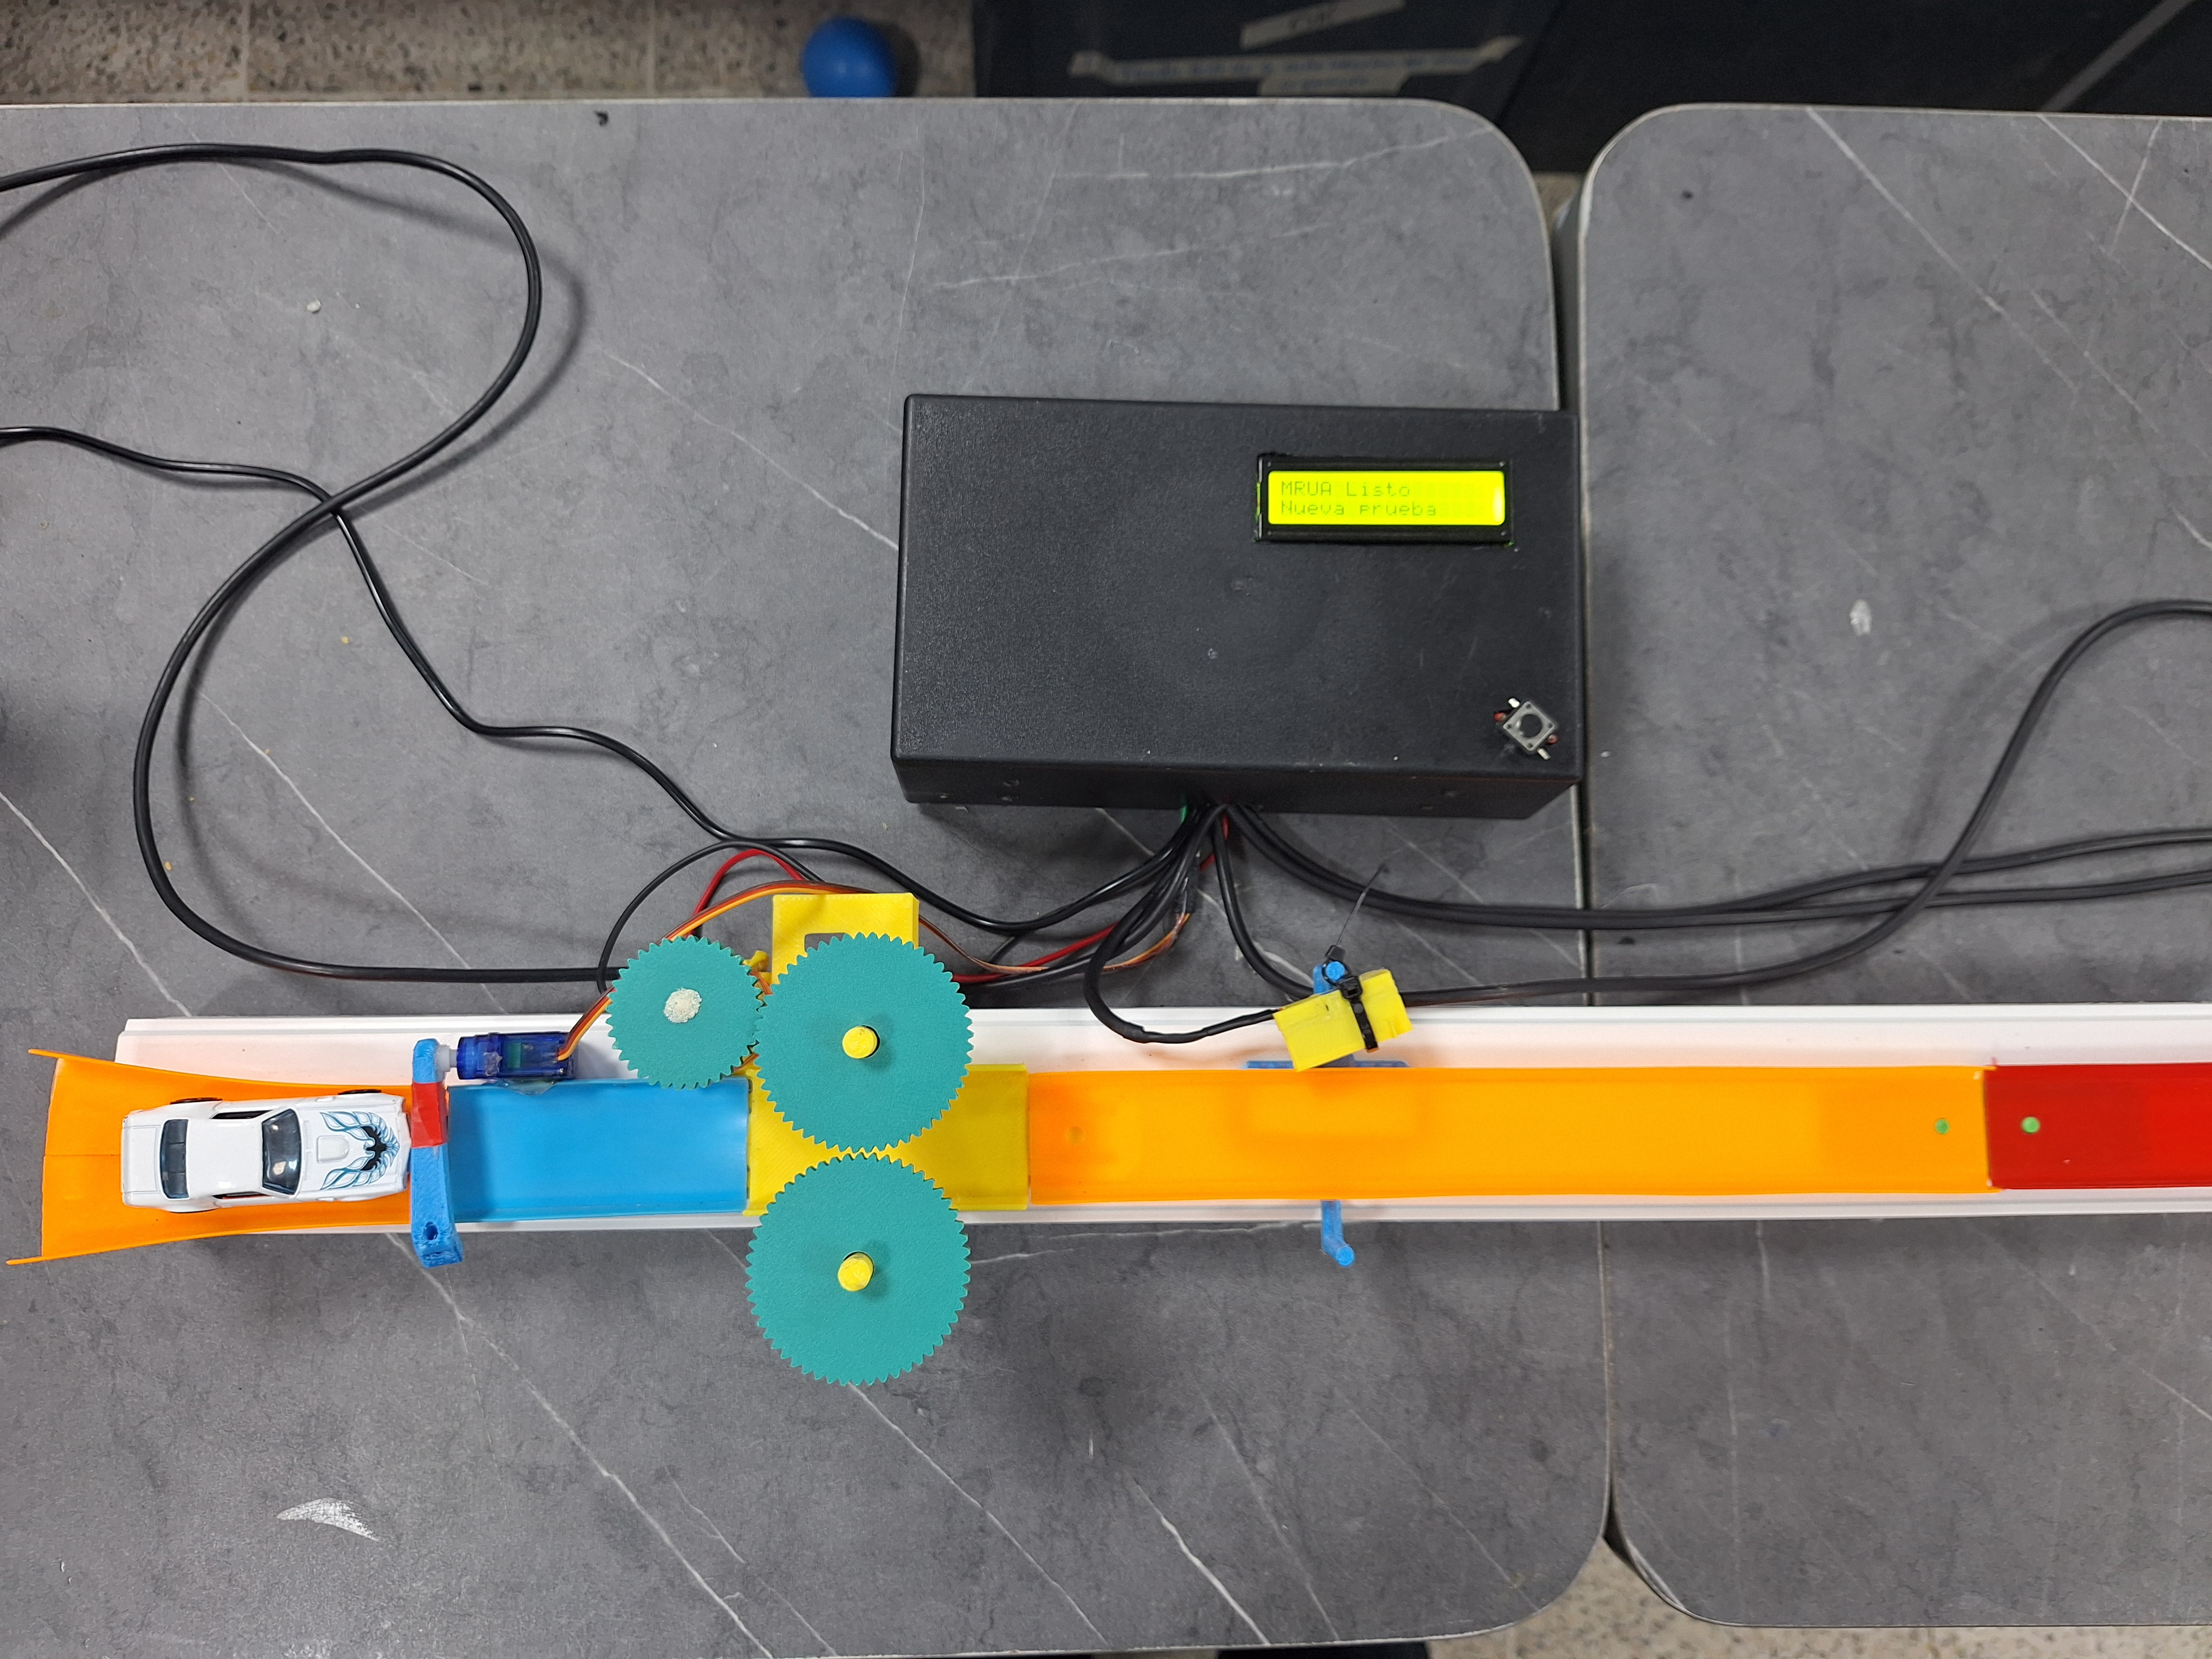
\includegraphics[width=0.45\textwidth]{figures/setup_overview_inicio.jpg}}
\hspace{0.5cm}
\subfloat[]{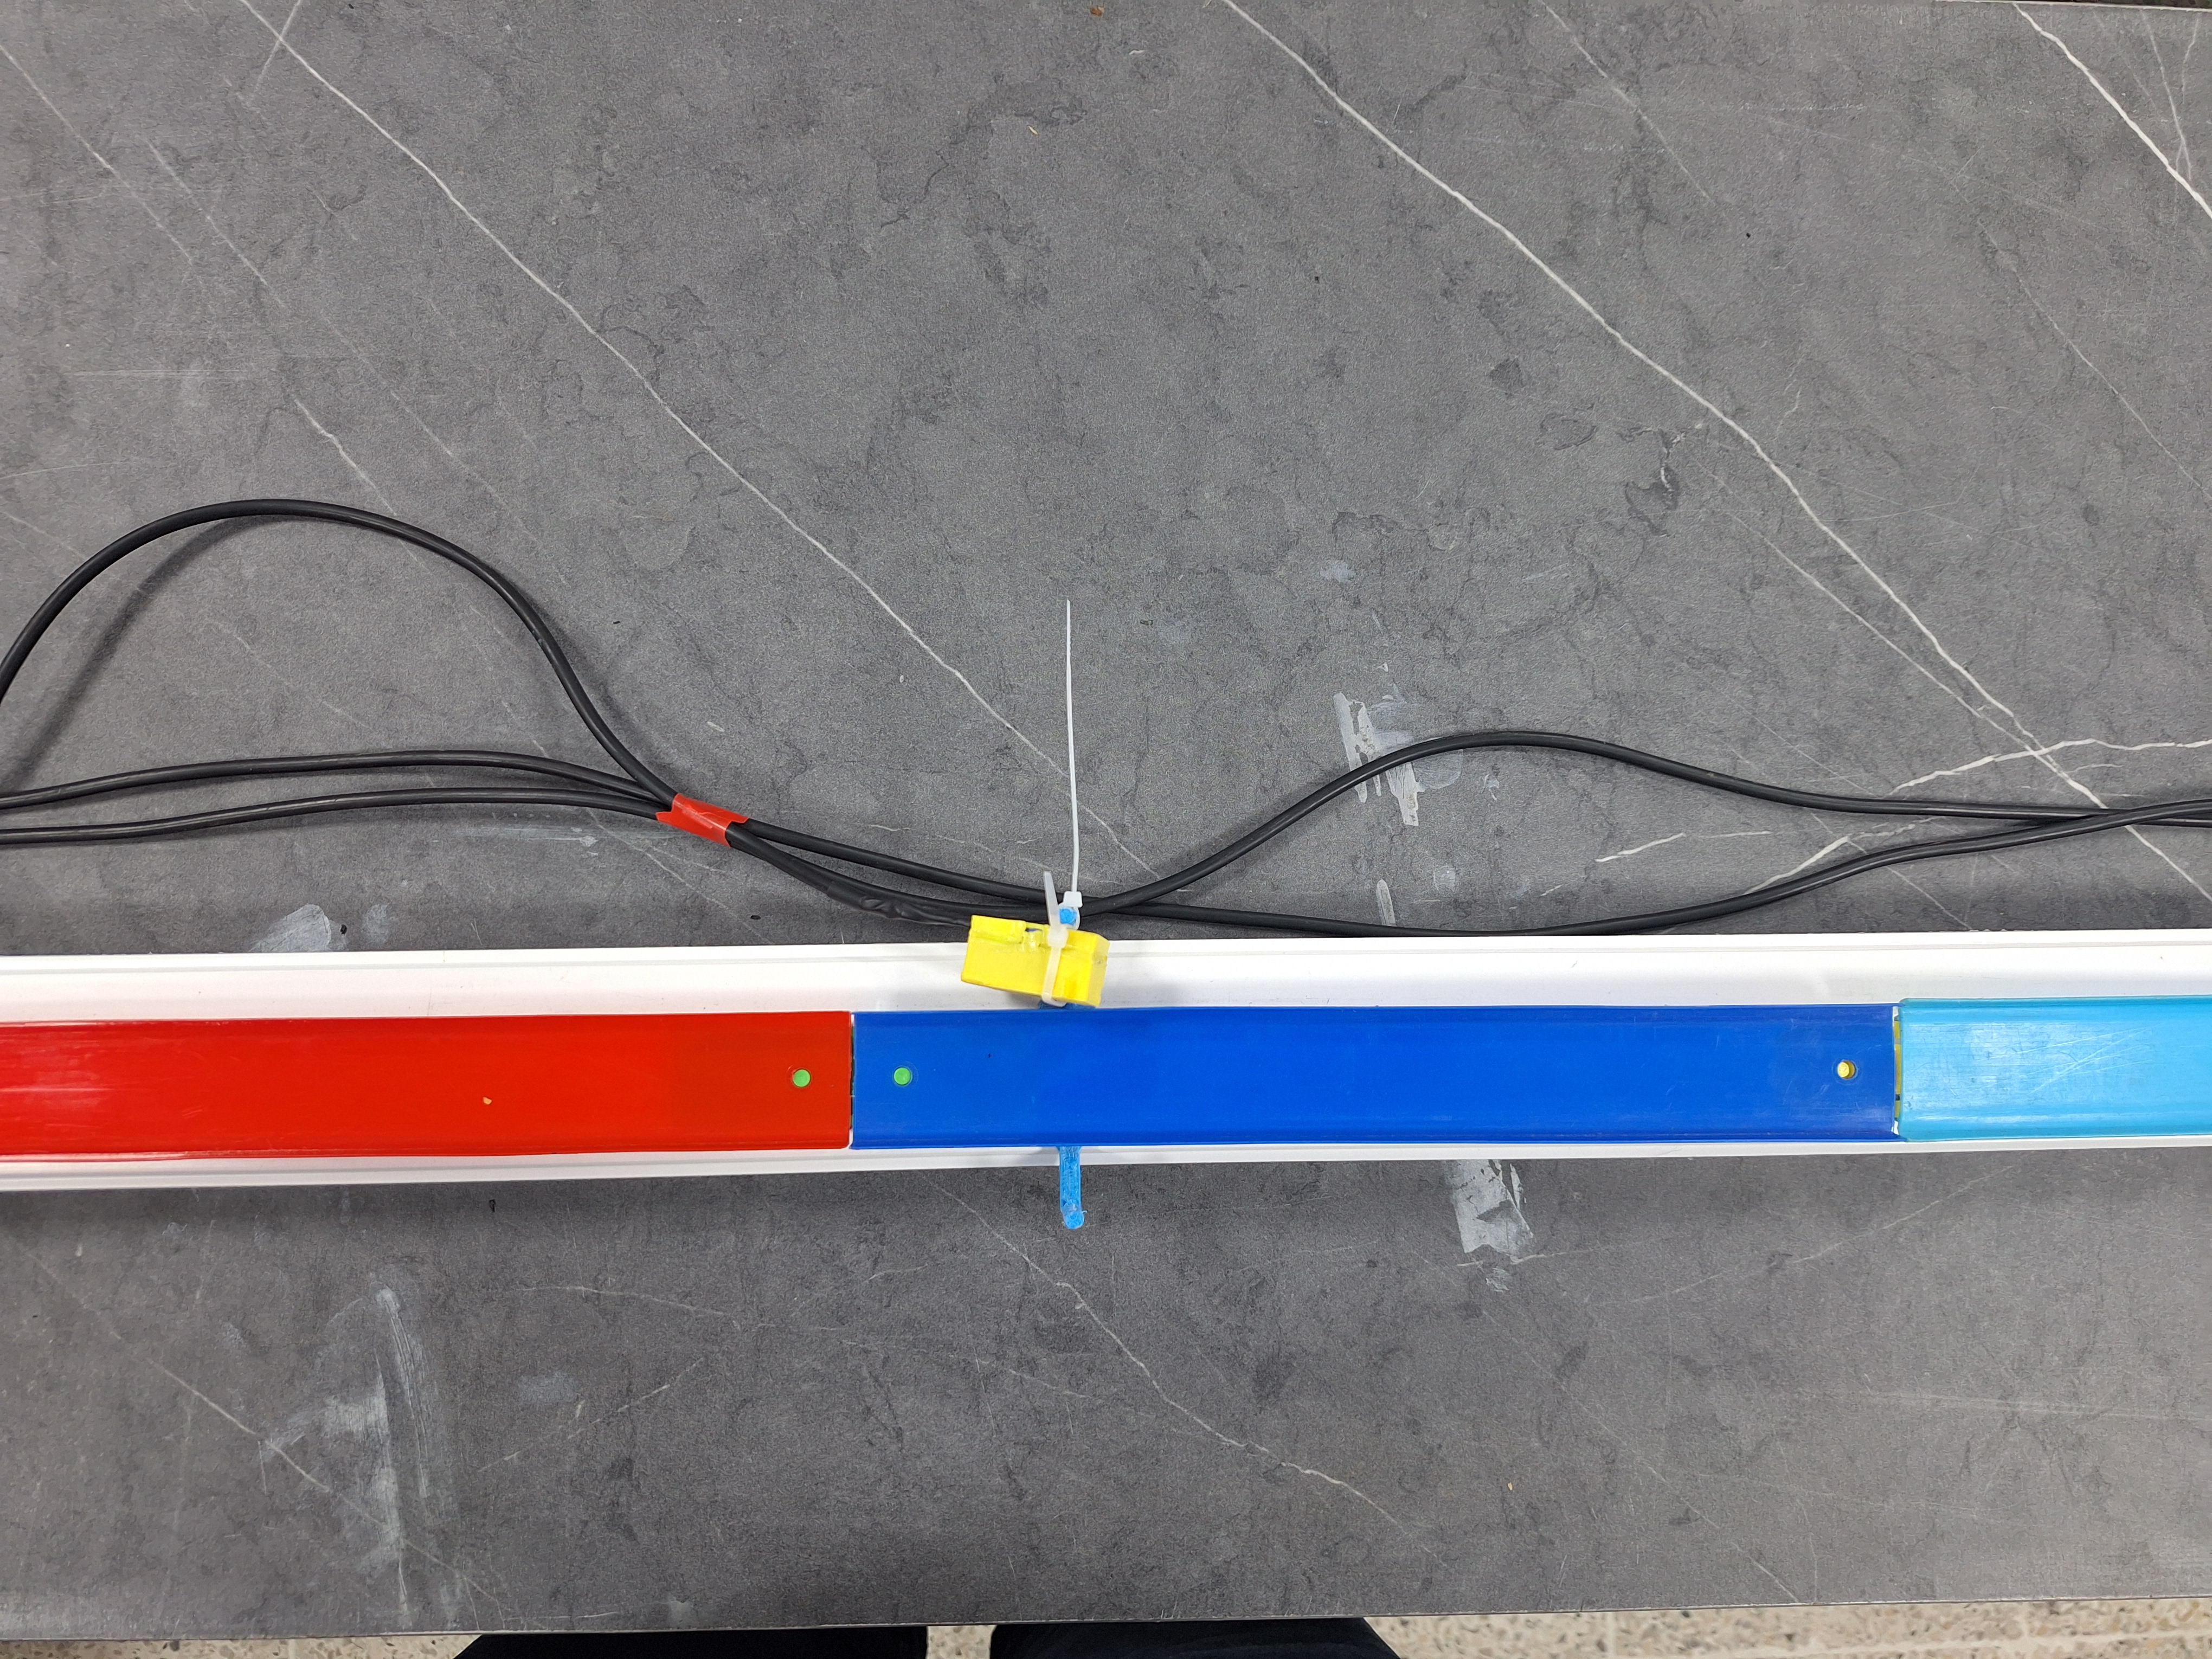
\includegraphics[width=0.45\textwidth]{figures/setup_overviewl_tramo2.jpg}}\\[0.3cm]
\subfloat[]{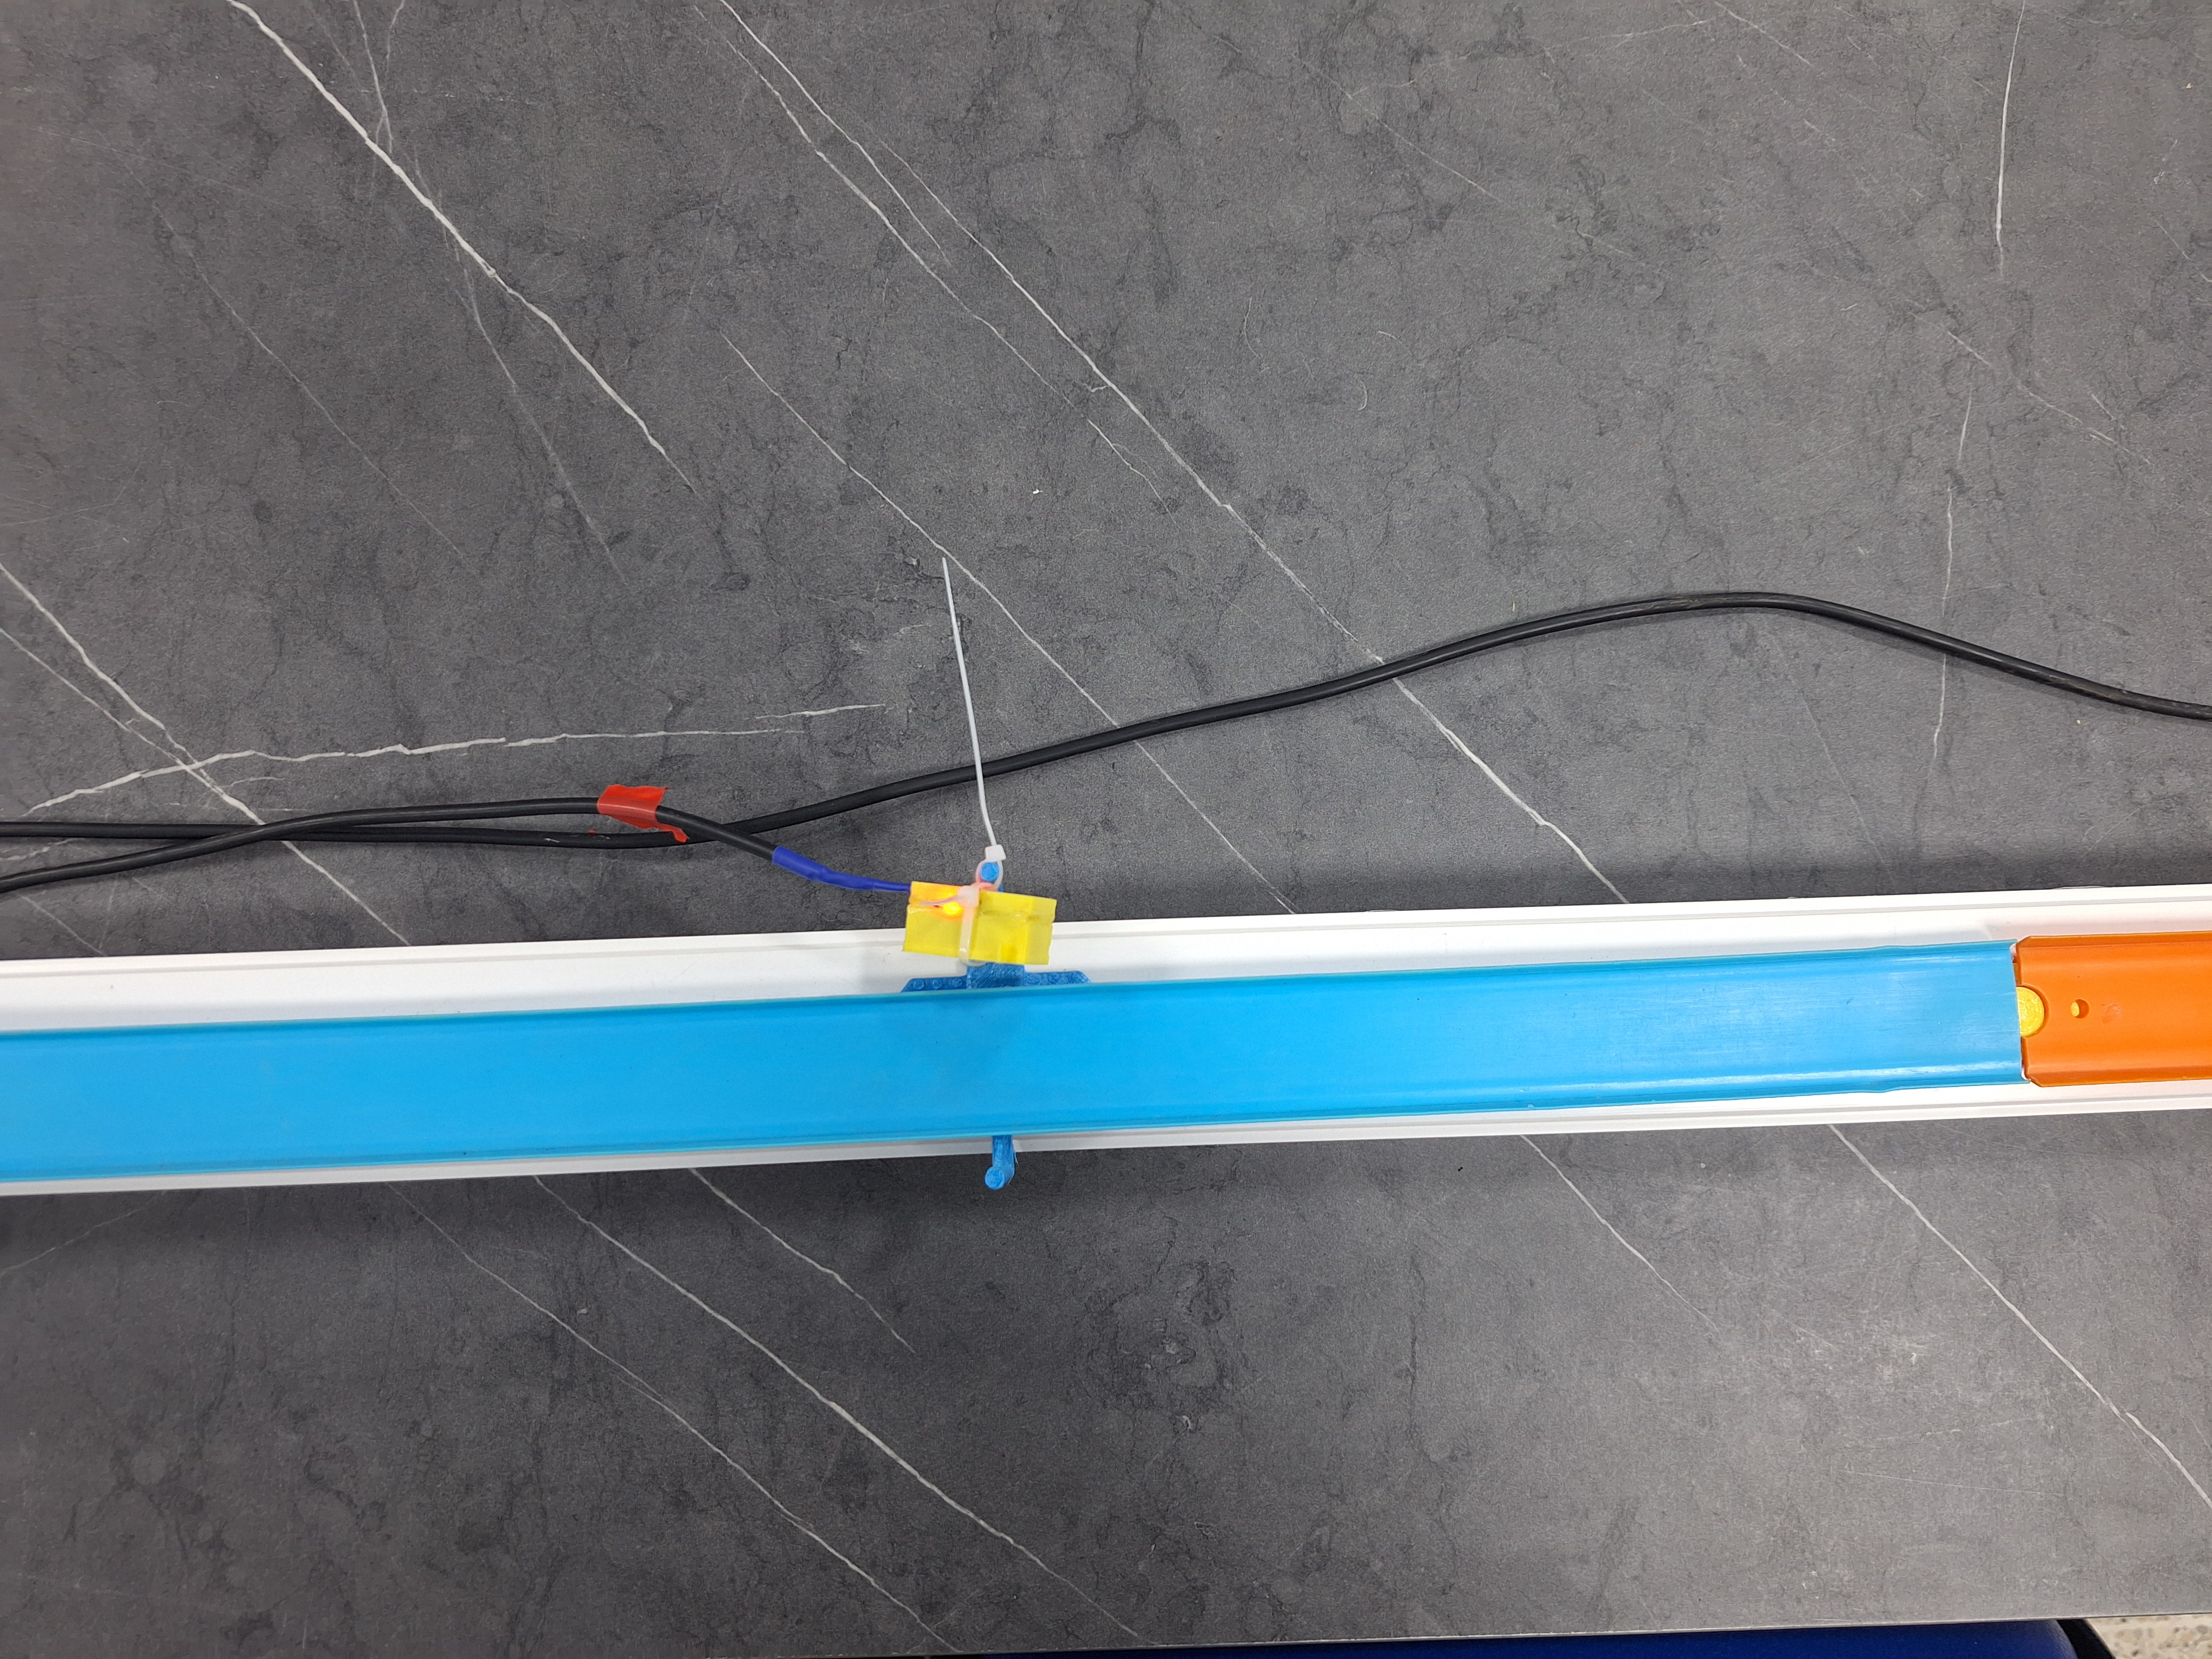
\includegraphics[width=0.45\textwidth]{figures/setup_overview_tramo3.jpg}}
\hspace{0.5cm}
\subfloat[]{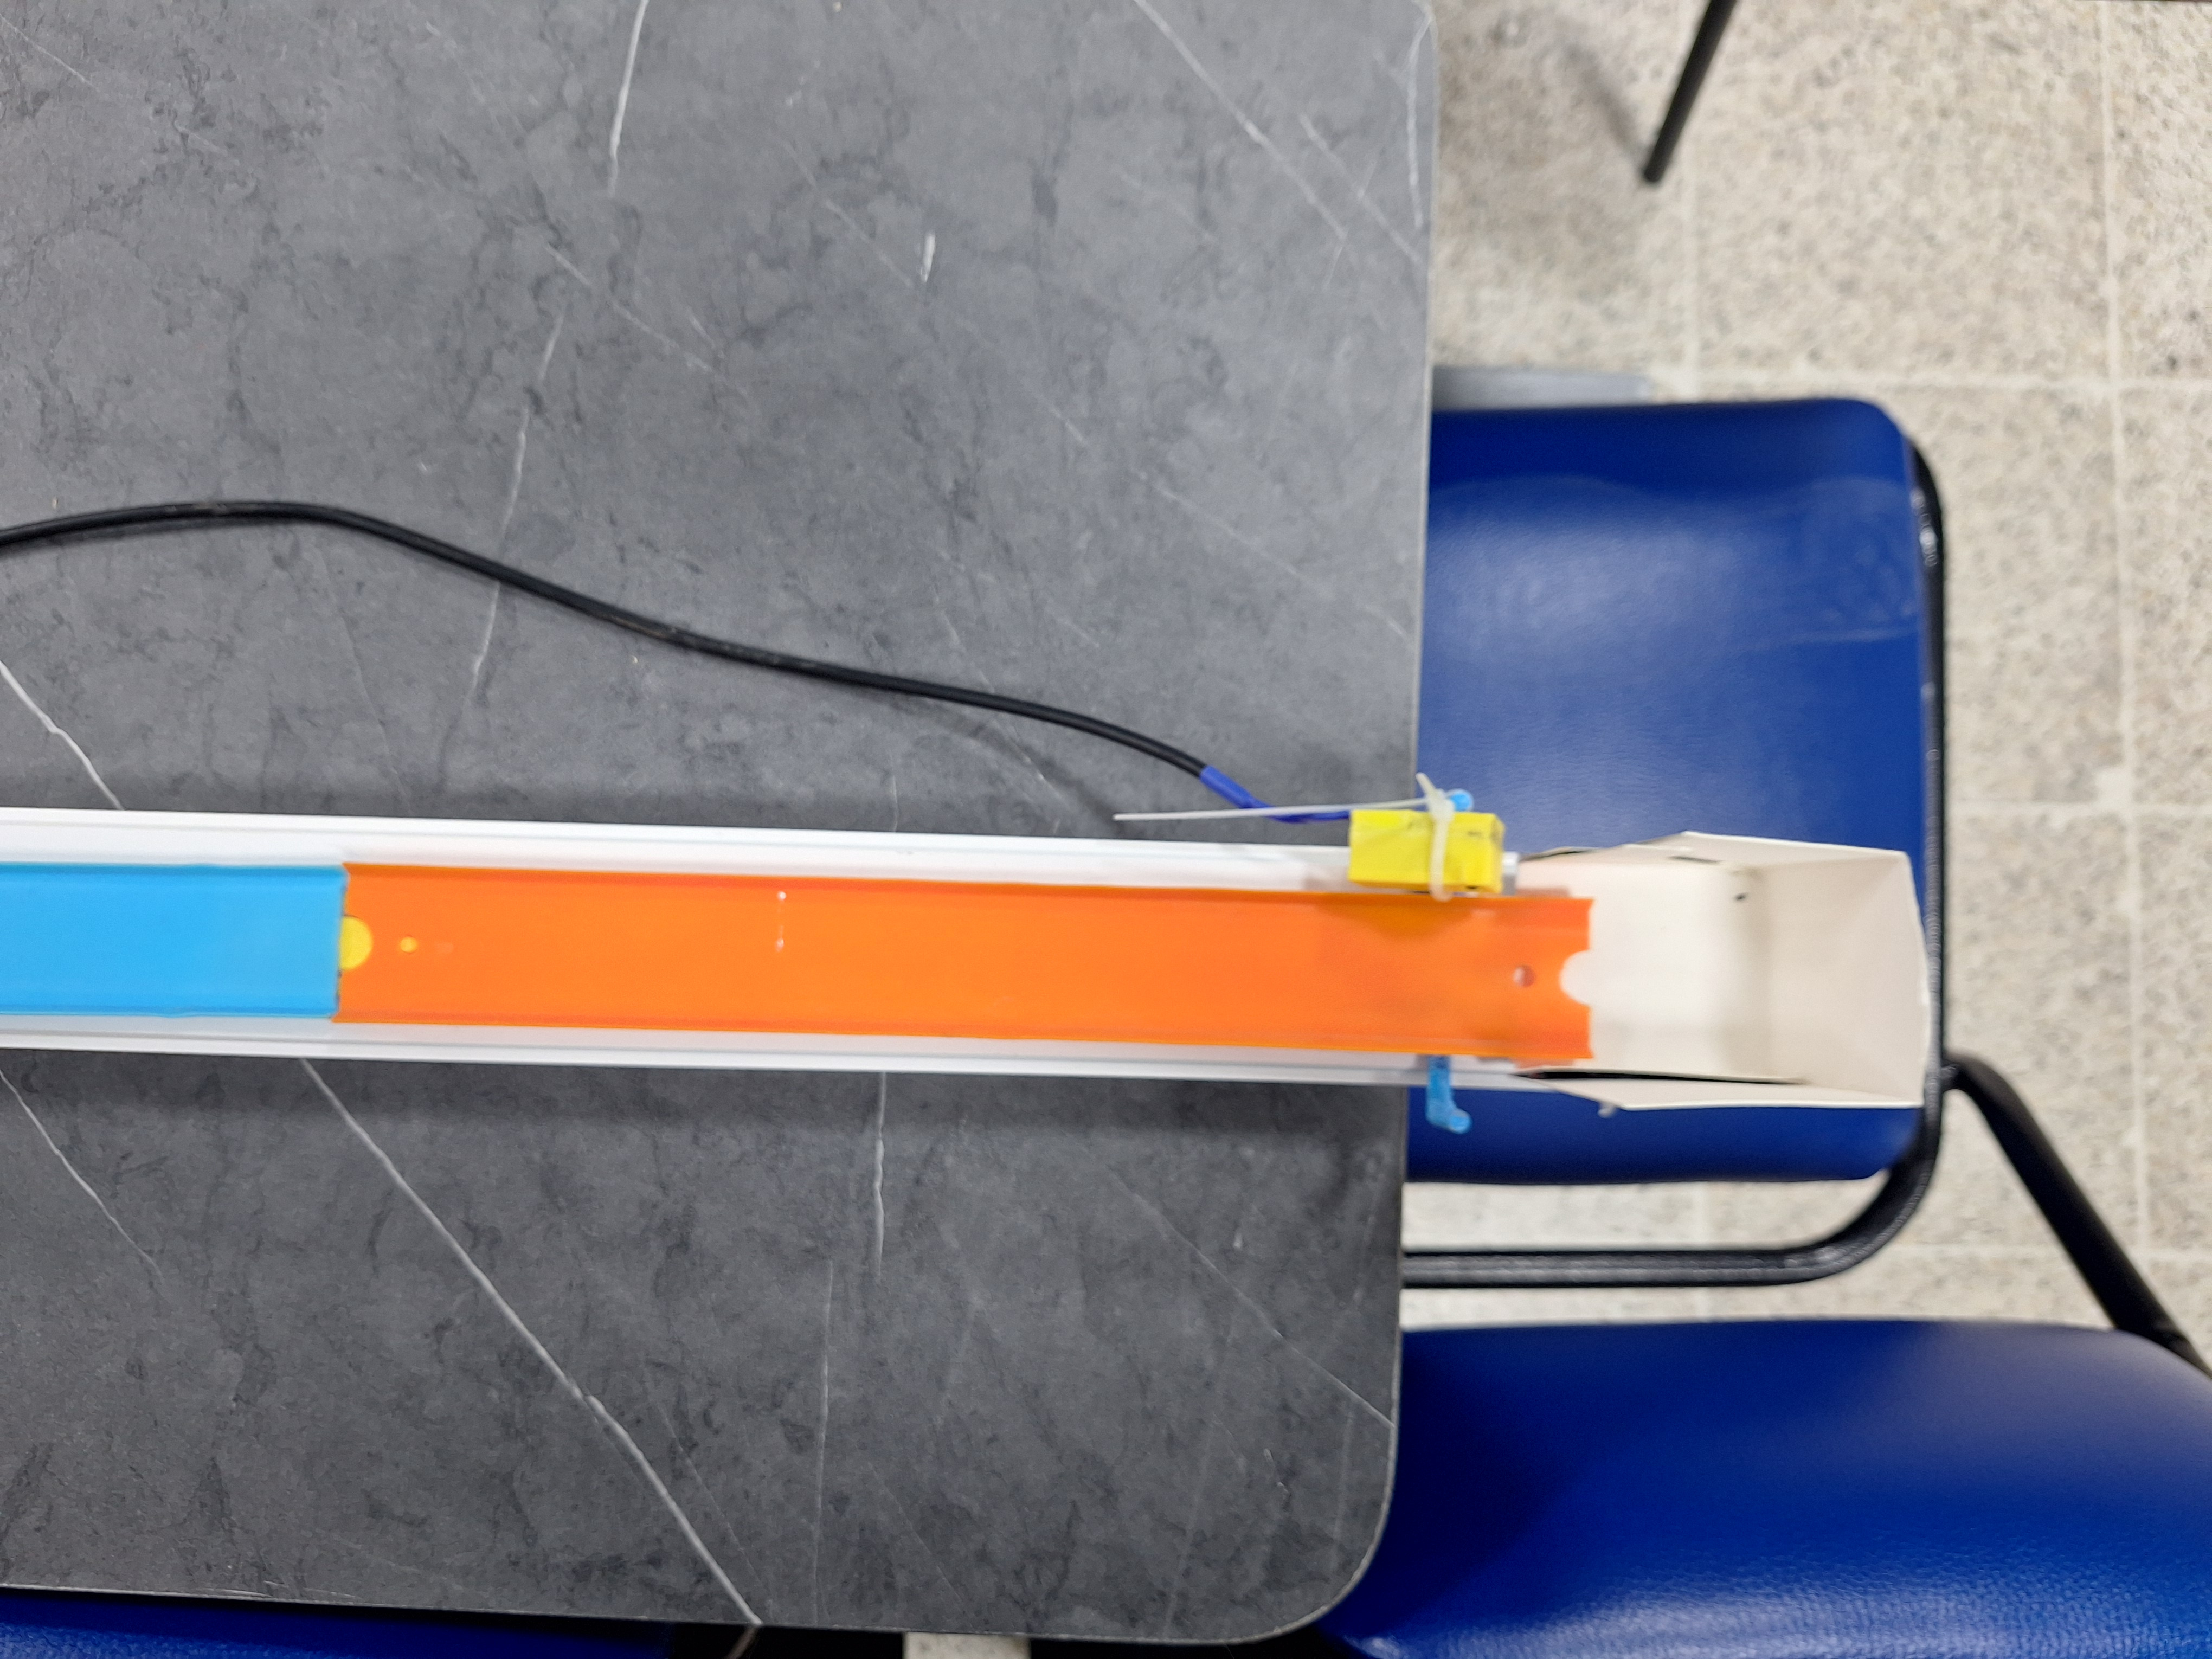
\includegraphics[width=0.45\textwidth]{figures/setup_overview_final.jpg}}
\caption{Secciones detalladas del montaje experimental: (a) inicio del recorrido; (b) tramo 2; (c) tramo 3; (d) punto de llegada y finalización del experimento.}
\label{fig:montaje_detalles}
\end{figure}

\begin{figure}[H]
\centering
\includegraphics[width=0.7\textwidth]{figures/setup_overview_completo.jpg}
\caption{Vista general del montaje experimental de MRUA basado en IoT.}
\label{fig:vista_general}
\end{figure}

Para facilitar la interacción remota con el experimento, se desarrolló una interfaz web de usuario que centraliza el control y la visualización del sistema. Como se muestra en la Figura~\ref{fig:interfaz_web}, esta plataforma permite al usuario iniciar y detener la secuencia experimental de manera controlada. Adicionalmente, la interfaz procesa los datos en tiempo real, generando automáticamente una gráfica con los resultados cinemáticos obtenidos tras cada ensayo. Para garantizar la supervisión visual del proceso, se integró una transmisión de video en vivo mediante una cámara, permitiendo corroborar el movimiento físico del carrito con los datos telemétricos recibidos.

\begin{figure}[H]
\centering
\includegraphics[width=0.7\textwidth]{figures/InterfazWeb.jpg}
\caption{Interfaz web desarrollada para el control y monitoreo remoto del experimento.}
\label{fig:interfaz_web}
\end{figure}


\subsection{Sensor S1: Inicio del movimiento}

El Sensor S1 corresponde al punto de partida del movimiento (\(t=0\)). En ambas modalidades, este sensor actúa como disparador temporal del experimento; por lo tanto, el tiempo registrado es sistemáticamente cero o muy cercano a cero.

\begin{table}[H]
	\caption{Resultados estadísticos para el Sensor S1.}
	\label{tab:s1_results}
	\centering
	\small
	\begin{tabular}{lccc}
		\toprule
		\textbf{Modalidad} & \textbf{\(\bar{x}\) (s)} & \textbf{\(s\) (s)} & \textbf{\(n\)} \\
		\midrule
		Presencial & 0.00 & 0.00 & 35 \\
		Remota     & 0.00 & 0.00 & 35 \\
		\bottomrule
	\end{tabular}
\end{table}

\begin{figure}[H]
    \centering
    \includegraphics[width=0.7\textwidth]{figures/correlation_sensor_S1.png}
    \caption{Gráfica de correlación para el Sensor S1 (Remota vs. Presencial).}
    \label{fig:corr_s1}
\end{figure}

Como se muestra en la Figura~\ref{fig:corr_s1}, los puntos de datos se concentran en el origen. El coeficiente de correlación es técnicamente indefinido o nulo (\(r \approx 0\)) porque la varianza de los datos es cero (\(s=0\)). Este comportamiento es físicamente esperado y confirma que S1 funciona correctamente como punto de referencia de sincronización tanto para el cronómetro manual como para el módulo de control digital. No hay fluctuaciones ni ruido experimental que afecten este estado inicial.

\subsection{Sensor S2: Primera sección intermedia}

El Sensor S2 se encuentra al final de la primera sección de la pista. Los resultados en la Tabla~\ref{tab:s2_results} muestran una alta consistencia entre las medias de ambas modalidades (1.17 s vs 1.19 s), con desviaciones estándar comparables (0.15 s vs 0.16 s).

\begin{table}[H]
	\caption{Resultados estadísticos para el Sensor S2.}
	\label{tab:s2_results}
	\centering
	\small
	\begin{tabular}{lccc}
		\toprule
		\textbf{Modalidad} & \textbf{\(\bar{x}\) (s)} & \textbf{\(s\) (s)} & \textbf{\(n\)} \\
		\midrule
		Presencial & 1.17 & 0.15 & 35 \\
		Remota     & 1.19 & 0.16 & 35 \\
		\bottomrule
	\end{tabular}
\end{table}

\begin{figure}[H]
    \centering
    \includegraphics[width=0.7\textwidth]{figures/correlation_sensor_S2.png}
    \caption{Gráfica de correlación para el Sensor S2 (Remota vs. Presencial).}
    \label{fig:corr_s2}
\end{figure}

La gráfica de la Figura~\ref{fig:corr_s2} presenta una distribución dispersa de puntos. El coeficiente de correlación calculado es bajo (\(r < 0.3\)), clasificando la correlación como nula o débil. Este resultado se interpreta físicamente por la independencia de los ensayos: dado que el "ensayo presencial 1" y el "ensayo remoto 1" son eventos físicos distintos separados en el tiempo, están sujetos a diferentes fluctuaciones aleatorias (fricción inicial de liberación, ligeras variaciones de resistencia del aire). La falta de correlación valida que el error de medición es aleatorio en lugar de sistemático; el sistema IoT no introduce un sesgo que lo aproxime o distancie esencialmente de la medición manual, sino que simplemente captura la variabilidad natural del fenómeno de MRUA.

\subsection{Sensor S3: Segunda sección intermedia}

El Sensor S3 captura el movimiento a una velocidad mayor. La Tabla~\ref{tab:s3_results} muestra tiempos medios muy similares para ambas modalidades (1.66 s vs 1.69 s), con desviaciones estándar comparables (0.23 s vs 0.24 s) que indican una precisión de medición consistente en ambos modos.

\begin{table}[H]
	\caption{Resultados estadísticos para el Sensor S3.}
	\label{tab:s3_results}
	\centering
	\small
	\begin{tabular}{lccc}
		\toprule
		\textbf{Modalidad} & \textbf{\(\bar{x}\) (s)} & \textbf{\(s\) (s)} & \textbf{\(n\)} \\
		\midrule
		Presencial & 1.66 & 0.23 & 35 \\
		Remota     & 1.69 & 0.24 & 35 \\
		\bottomrule
	\end{tabular}
\end{table}

\begin{figure}[H]
    \centering
    \includegraphics[width=0.7\textwidth]{figures/correlation_sensor_S3.png}
    \caption{Gráfica de correlación para el Sensor S3 (Remota vs. Presencial).}
    \label{fig:corr_s3}
\end{figure}

La Figura~\ref{fig:corr_s3} muestra nuevamente una nube de puntos con baja correlación. El valor débil de \(r\) se atribuye al ruido experimental acumulado. A medida que el carrito se mueve más lejos, las pequeñas variaciones iniciales en la aceleración se acumulan en desviaciones mayores de posición/tiempo. El hecho de que tanto el sistema remoto como el presencial muestren desviaciones estándar casi idénticas (\(s=0.23\) s vs \(s=0.24\) s) demuestra que la detección automatizada del módulo de control se desempeña de manera comparable al cronometraje manual, capturando la variabilidad natural del fenómeno de MRUA con precisión similar.

\subsection{Sensor S4: Final de la pista}

El Sensor S4 representa el punto de medición final, donde la velocidad es máxima. Los resultados muestran un excelente acuerdo entre ambas modalidades, con tiempos medios prácticamente idénticos (2.05 s vs 2.04 s) y desviaciones estándar comparables (0.28 s vs 0.29 s).

\begin{table}[H]
	\caption{Resultados estadísticos para el Sensor S4.}
	\label{tab:s4_results}
	\centering
	\small
	\begin{tabular}{lccc}
		\toprule
		\textbf{Modalidad} & \textbf{\(\bar{x}\) (s)} & \textbf{\(s\) (s)} & \textbf{\(n\)} \\
		\midrule
		Presencial & 2.05 & 0.28 & 35 \\
		Remota     & 2.04 & 0.29 & 35 \\
		\bottomrule
	\end{tabular}
\end{table}

\begin{figure}[H]
    \centering
    \includegraphics[width=0.7\textwidth]{figures/correlation_sensor_S4.png}
    \caption{Gráfica de correlación para el Sensor S4 (Remota vs. Presencial).}
    \label{fig:corr_s4}
\end{figure}

El análisis de la Figura~\ref{fig:corr_s4} confirma el patrón observado en los sensores anteriores. Tanto las mediciones presenciales como remotas muestran una dispersión comparable (\(s=0.28\) s y \(s=0.29\) s respectivamente), con tiempos medios prácticamente idénticos (2.05 s vs 2.04 s). El coeficiente de correlación bajo es consistente con la independencia de los ensayos; cada medición captura la variabilidad natural del fenómeno de MRUA bajo diferentes condiciones iniciales. El notable acuerdo entre ambas modalidades demuestra que el sistema de \textit{retrofitting} IoT replica exitosamente las capacidades de medición de la configuración tradicional, proporcionando datos cinemáticos confiables adecuados para el análisis cuantitativo del movimiento uniformemente acelerado.

%-------------------------------------------------
% DISCUSION
%-------------------------------------------------

\section{Discussion}

\subsection{Interpretation of Temporal and Kinematic Results}

Los resultados obtenidos demuestran que el sistema de \textit{retrofitting} IoT es capaz de capturar la dinámica del experimento de MRUA con una fidelidad comparable e incluso superior en estabilidad a la del montaje presencial tradicional. Contrario a lo esperado para sistemas distribuidos, las mediciones en la modalidad remota presentaron una dispersión controlada, lo que evidencia la eficiencia del manejo de interrupciones en el módulo de control. La consistencia de los datos sugiere que la latencia de red, aunque presente, no degradó la calidad de la recolección de datos cinemáticos gracias al sellado temporal local.

\subsection{Implications for IoT-Based Retrofitting of Physics Laboratories}

La viabilidad técnica del modelo propuesto tiene implicaciones directas para la modernización de infraestructuras educativas con recursos limitados. El enfoque de \textit{retrofitting} demuestra que es posible transformar equipamiento clásico en activos digitales conectados sin necesidad de sustituir la instrumentación original. La arquitectura modular adoptada permite una escalabilidad eficiente, donde la capa de sensórica y control se desacopla de los servicios de visualización y almacenamiento. Los resultados validan que las soluciones de bajo coste basadas en hardware masivo pueden alcanzar niveles de precisión adecuados para fines académicos, facilitando la transición hacia entornos de aprendizaje híbridos que no dependen exclusivamente de la presencia física en el laboratorio.

\subsection{Comparison with Related Works}

Al contrastar los resultados con la literatura previa, se observan similitudes fundamentales con los trabajos de Viswanadh \textit{et al.} \cite{r2} y Lustig \textit{et al.} \cite{r5} en cuanto a la efectividad de las arquitecturas modulares para experimentos remotos. Sin embargo, el presente estudio aporta una validación cuantitativa específica para el caso del MRUA, extendiendo las propuestas de Guerrero-Osuna \textit{et al.} \cite{r4} y Fuertes \textit{et al.} \cite{r3}, quienes se centraron primordialmente en el control de motores. A diferencia de las soluciones basadas en SmartIPLs revisadas por Zhao \cite{r6}, que dependen de sensores internos de teléfonos inteligentes, el sistema implementado ofrece una infraestructura fija y dedicada que garantiza una mayor repetibilidad en las condiciones de ensayo, manteniendo la accesibilidad económica del montaje.

\subsection{Limitations of the Study}

A pesar del desempeño satisfactorio del prototipo, se identifican limitaciones intrínsecas en el alcance de la investigación. En primer lugar, aunque la estabilidad fue alta, el sistema sigue dependiendo de la disponibilidad continua del servidor MQTT para la transmisión de datos en tiempo real. En segundo lugar, el número de ensayos realizados (n=35 por modalidad), aunque robusto, se limita a un entorno controlado de laboratorio universitario. Asimismo, el experimento se desarrolla bajo condiciones mecánicas donde factores como la fricción residual del carrito y la alineación micrométrica de los sensores ópticos introducen variaciones físicas que son independientes de la instrumentación IoT.

\subsection{Future Work}

Las futuras líneas de investigación se orientan hacia la optimización de la capa de percepción y la robustez del sistema. Se propone la integración de sensores de mayor resolución temporal y el uso de protocolos de comunicación con priorización de tráfico para minimizar el impacto de la latencia de red. Asimismo, resulta pertinente incrementar el volumen de ensayos para robustecer el análisis estadístico y realizar mediciones explícitas de la latencia en cada etapa de la cadena de datos. Desde una perspectiva funcional, el sistema puede expandirse para instrumentar otros experimentos de dinámica y energía, integrando los flujos de datos con plataformas educativas de gestión de aprendizaje (LMS) para automatizar la evaluación de las prácticas experimentales.

\section{Conclusions}

El presente estudio ha validado con éxito la eficacia del \textit{retrofit} de laboratorios de física mediante tecnologías IoT de bajo coste. a través de una extensa campaña experimental con 70 ensayos (35 presenciales y 35 remotos), se demostró que la arquitectura propuesta basada en el módulo de control y sensores infrarrojos es capaz de replicar la dinámica del MRUA con una fidelidad comparable, e incluso superior en términos de estabilidad, a la del montaje tradicional.

Los resultados cuantitativos demuestran que no existe una degradación significativa de la precisión debido a la operación remota. Por el contrario, la modalidad remota exhibió una consistencia notable, con desviaciones estándar controladas en las mediciones críticas de velocidad y aceleración. La implementación de la interfaz web jugó un papel crucial, no solo como panel de control, sino como herramienta pedagógica que integra la visualización de datos en tiempo real y la verificación visual mediante video, enriqueciendo la experiencia de aprendizaje.

En conclusión, este trabajo confirma que la digitalización de experimentos clásicos no requiere inversiones masivas en equipamiento propietario. La metodología de \textit{retrofitting} presentada ofrece una ruta escalable y sostenible para democratizar el acceso a la educación experimental de alta calidad, permitiendo a las instituciones educativas maximizar la utilidad de sus recursos existentes en el contexto de modelos híbridos de enseñanza.

%-------------------------------------------------
% REFERENCIAS
%-------------------------------------------------

\reftitle{References}
\begin{thebibliography}{999}

\bibitem{r1}
Lahme, S.Z.; Klein, P.; Lehtinen, A.; M\"uller, A.; Pirinen, P.; Ron\v{c}evi\'c, L.; Su\v{s}ac, A. 
Physics lab courses under digital transformation: A trinational survey among university lab instructors about the role of new digital technologies and learning objectives. 
\textit{Phys. Rev. Phys. Educ. Res.} \textbf{2023}, \textit{19}, 020159. 
\href{https://doi.org/10.1103/PhysRevPhysEducRes.19.020159}{doi:10.1103/PhysRevPhysEducRes.19.020159}.

\bibitem{r2}
Viswanadh, K.S.; Gureja, A.; Walchatwar, N.; Agrawal, R.; Sinha, S.; 
Chaudhari, S.; Vaidhyanathan, K.; Hussain, A.M. 
Engineering End-to-End Remote Labs Using IoT-Based Retrofitting. 
\textit{IEEE Access} \textbf{2024}, \textit{PP}, 1--1. 
\href{https://doi.org/10.1109/ACCESS.2024.3523066}{doi:10.1109/ACCESS.2024.3523066}.

\bibitem{r3}
Fuertes, J.J.; Mart\'inez, J.M.; Dormido, S.; Vargas, H.; 
S\'anchez, J.; Duro, N. 
Virtual and Remote Laboratory of a DC Motor for Learning Control Theory. 
\textit{Int. J. Eng. Educ.} \textbf{2011}, \textit{27}, 1--12.

\bibitem{r4}
Guerrero-Osuna, H.A.; Garc\'ia-V\'azquez, F.A.; Ibarra-Delgado, S.; Sol\'is-S\'anchez, L.O. 
Developing a Cloud and IoT-Integrated Remote Laboratory to Enhance Education 4.0: 
An Approach for FPGA-Based Motor Control. 
\textit{Appl. Sci.} \textbf{2024}, \textit{14}, 10115.

\bibitem{r5}
Lustig, F.; Kuri\v{s}\v{c}\'ak, P.; Brom, P.; Dvo\v{r}\'ak, J. 
Open Modular Hardware and Software Kit for Creations of Remote Experiments Accessible from PC and Mobile Devices. 
\textit{Int. J. Online Eng. (iJOE)} \textbf{2016}, \textit{12}, 30--36. 
\href{https://doi.org/10.3991/ijoe.v12i07.5833}{doi:10.3991/ijoe.v12i07.5833}.

\bibitem{r6}
Zhao, Y. 
Smartphone-Based Undergraduate Physics Labs: A Comprehensive Review. 
\textit{IEEE Access} \textbf{2024}, \textit{13}, 1106--1132. 
\href{https://doi.org/10.1109/ACCESS.2024.3523066}{doi:10.1109/ACCESS.2024.3523066}.

\bibitem{r7}
Dizdarevic, J.; Jukan, A.
Engineering an IoT--Edge--Cloud Computing System Architecture: Lessons Learnt from an Undergraduate Laboratory Course.
\textit{IoT} \textbf{2022}, \textit{3}, 145--163.
\href{https://doi.org/10.3390/iot3010010}{doi:10.3390/iot3010010}.

\bibitem{r8}
Azad, A.K.M.
Use of Internet of Things for Remote Laboratory Settings.
\textit{IoT} \textbf{2021}, \textit{2}, 203--232.
\href{https://doi.org/10.3390/iot2020011}{doi:10.3390/iot2020011}.

\bibitem{r9}
Palmer, C.; Roullier, B.; Aamir, M.; McQuade, F.; Stella, L.; Anjum, A.
Digital Twinning Remote Laboratories for Online Practical Learning.
\textit{Sensors} \textbf{2022}, \textit{22}, 2351.
\href{https://doi.org/10.3390/s22062351}{doi:10.3390/s22062351}.

\bibitem{r10}
Atzori, L.; Iera, A.; Morabito, G. 
The Internet of Things: A survey. 
\textit{Comput. Netw.} \textbf{2010}, \textit{54}, 2787--2805. 
\href{https://doi.org/10.1016/j.comnet.2010.05.010}{doi:10.1016/j.comnet.2010.05.010}.

\bibitem{r11}
Hevner, A.R.; March, S.T.; Park, J.; Ram, S. 
Design Science in Information Systems Research. 
\textit{MIS Q.} \textbf{2004}, \textit{28}, 75--105.

\bibitem{r12}
ISO/IEC. 
\textit{ISO/IEC 15288:2015 Systems and Software Engineering—System Life Cycle Processes}; 
International Organization for Standardization: Geneva, Switzerland, 2015.

\bibitem{r13}
Mattel, Inc.
\textit{Hot Wheels Track Sets}.
Available online: \url{https://shop.mattel.com/pages/hot-wheels} (accessed on 5 December 2025).

\bibitem{r14}
Mattel, Inc.
\textit{Hot Wheels Cars}.
Available online: \url{https://shop.mattel.com/collections/hot-wheels-cars} (accessed on 5 December 2025).

\bibitem{r15}
Vishay Intertechnology, Inc.
\textit{TCRT5000 Reflective Optical Sensor}.
Available online: \url{https://www.vishay.com/docs/83751/tcrt5000.pdf} (accessed on 5 December 2025).

\bibitem{r16}
Espressif Systems.
\textit{ESP32-WROOM-32 Datasheet}.
Available online: \url{https://www.espressif.com/sites/default/files/documentation/esp32-wroom-32_datasheet_en.pdf} (accessed on 5 December 2025).

\bibitem{r17}
Thingiverse.
\textit{Mechanical Support for Track-Based Experiments (Thing 3630616)}.
Available online: \url{https://www.thingiverse.com/thing:3630616}
(accessed on 5 December 2025).

\bibitem{r18}
Thingiverse.
\textit{3D Printed Modular Track Components (Thing 3485484)}.
Available online: \url{https://www.thingiverse.com/thing:3485484}
(accessed on 5 December 2025).

\bibitem{r19}
Thingiverse.
\textit{3D Printed Structural Reinforcement Parts (Thing 4381935)}.
Available online: \url{https://www.thingiverse.com/thing:4381935}
(accessed on 5 December 2025).

\bibitem{r20}
Thingiverse.
\textit{3D Printed Mechanical Pusher Mechanism (Thing 2806324)}.
Available online: \url{https://www.thingiverse.com/thing:2806324}
(accessed on 5 December 2025).

\bibitem{r21}
Tower Pro.
\textit{SG90 Micro Servo Motor Datasheet}.
Available online: \url{http://www.ee.ic.ac.uk/pjs99/projects/servo/sg90_datasheet.pdf} (accessed on 5 December 2025).

\bibitem{r22}
StepperOnline.
\textit{NEMA 17 Stepper Motor Bipolar Datasheet}.
Available online: \url{https://www.omc-stepperonline.com/download/17HS19-2004S1.pdf} (accessed on 5 December 2025).

\bibitem{r23}
STMicroelectronics.
\textit{L298N Dual H-Bridge Motor Driver Datasheet}.
Available online: \url{https://www.st.com/resource/en/datasheet/l298.pdf} (accessed on 5 December 2025).

\bibitem{r24}
Generic Electronics Suppliers.
\textit{LCD 20x4 Display with I\textsuperscript{2}C Interface Datasheet}.
Available online: \url{https://www.sparkfun.com/datasheets/LCD/HD44780.pdf} (accessed on 5 December 2025).

\bibitem{r25}
Generic Electronics Suppliers.
\textit{Tactile Push Button Switch for Breadboard}.
Available online: \url{https://www.adafruit.com/product/367} (accessed on 5 December 2025).

\bibitem{r26}
USB Implementers Forum.
\textit{USB Type-C Cable Specification}.
Available online: \url{https://www.usb.org/sites/default/files/USB%20Type-C%20Spec%20R2.0%20-%20August%202019.pdf} (accessed on 5 December 2025).

\bibitem{r27}
IEEE.
\textit{IEEE Standard for Wireless LAN Medium Access Control (MAC) and Physical Layer (PHY) Specifications}.
Available online: \url{https://ieeexplore.ieee.org/document/9363693} (accessed on 5 December 2025).

\bibitem{r28}
Generic Electronics Suppliers.
\textit{Dupont Jumper Wires (Male-Female and Female-Female)}.
Available online: \url{https://www.adafruit.com/category/289} (accessed on 5 December 2025).

\bibitem{r29}
Generic Electronics Suppliers.
\textit{Plastic Project Enclosure Box (135x75x40 mm)}.
Available online: \url{https://www.digikey.com/en/products/filter/enclosures/287} (accessed on 5 December 2025).

\bibitem{r30}
Generic Electronics Suppliers.
\textit{AC-DC Power Adapter 12V/1A}.
Available online: \url{https://www.digikey.com/en/products/filter/power-supplies-external-internal-off-board/171} (accessed on 5 December 2025).

\bibitem{r31}
Insta360.
\textit{Insta360 Link---4K AI Webcam Technical Specifications}.
Available online: \url{https://onlinemanual.insta360.com/link/en-us/introduction} (accessed on 5 December 2025).

\bibitem{r32}
Raspberry Pi Ltd.
\textit{Raspberry Pi 4 Model B Product Brief}.
Available online: \url{https://datasheets.raspberrypi.com/rpi4/raspberry-pi-4-product-brief.pdf} (accessed on 5 December 2025).

\bibitem{r33}
EMQ Technologies Co., Ltd.
\textit{EMQX---MQTT Platform for IoT Data Streaming Documentation}.
Available online: \url{https://docs.emqx.com/en/emqx/v5.0/} (accessed on 5 December 2025).

\bibitem{r34}
EMQ Technologies Co., Ltd.
\textit{MQTTX: Your All-in-One MQTT Client Toolbox Documentation}.
Available online: \url{https://mqttx.app/docs} (accessed on 5 December 2025).

\bibitem{r35}
OpenJS Foundation.
\textit{Node.js API Documentation}.
Available online: \url{https://nodejs.org/api/} (accessed on 5 December 2025).

\bibitem{r36}
OpenJS Foundation.
\textit{Express API Reference}.
Available online: \url{https://expressjs.com/en/4x/api.html} (accessed on 5 December 2025).

\bibitem{r37}
MongoDB, Inc.
\textit{MongoDB Documentation}.
Available online: \url{https://www.mongodb.com/docs/manual/} (accessed on 5 December 2025).

\bibitem{r38}
Mongoose.
\textit{Mongoose ODM API Documentation}.
Available online: \url{https://mongoosejs.com/docs/api.html} (accessed on 5 December 2025).

\bibitem{r39}
Vercel, Inc.
\textit{Next.js Documentation}.
Available online: \url{https://nextjs.org/docs} (accessed on 5 December 2025).

\bibitem{r40}
Meta Platforms, Inc.
\textit{React Reference Documentation}.
Available online: \url{https://react.dev/reference/react} (accessed on 5 December 2025).

\bibitem{r41}
Arduino AG.
\textit{Arduino IDE 2.x Documentation}.
Available online: \url{https://www.arduino.cc/en/software} (accessed on 5 December 2025).

\bibitem{r42}
Python Software Foundation.
\textit{Python 3 Documentation}.
Available online: \url{https://docs.python.org/3/} (accessed on 5 December 2025).

\bibitem{r43}
Eraser Labs, Inc.
\textit{Eraser---AI Co-Pilot for Technical Design and Documentation}.
Available online: \url{https://www.eraser.io} (accessed on 5 December 2025).

\bibitem{r44}
OpenAI. \textit{ChatGPT}.
Available online: \url{https://chat.openai.com} (accessed on 23 January 2026). Content generated with the assistance of ChatGPT.

\bibitem{r45}
Santiago Sosa Mej\'ia.
\textit{RemotePhysicsLab: Prototipo de laboratorio de f\'isica h\'ibrido basado en IoT}. 
Repositorio GitHub. 
Available online: \url{https://github.com/waltersosa/RemotePhysicsLab.git} (accessed on 5 December 2025).

\end{thebibliography}

\end{document}